\documentclass{article}
\usepackage[utf8]{inputenc}
\usepackage{hyperref}
\usepackage[T1]{fontenc}
\usepackage{lmodern}
\usepackage{layouts}
\usepackage[english]{babel}
\usepackage{microtype}
\usepackage{csquotes}

% Page layout
\usepackage{fancyhdr}
\usepackage[a4paper,width=150mm,top=30mm,bottom=30mm]{geometry}
\usepackage{multicol}
\setlength{\columnsep}{1cm}
\usepackage{changepage}

\pagestyle{fancy}
\fancyhf{}
\lhead{Marco Ballarin}
\rhead{\today}
\cfoot{Homework 1, Neural Network and Deep Learning 2020/21 \\  \thepage}
\renewcommand{\headrulewidth}{2pt}
\renewcommand{\footrulewidth}{1pt}

% Physics and math
\usepackage{physics}
\usepackage{amsmath}
\usepackage{amssymb}
\usepackage[sorting=none]{biblatex}
\addbibresource{bibliography.bib}

% Images
\usepackage{graphics}
\usepackage{pgfplots}
\pgfplotsset{compat=1.16}
\usepackage{xcolor}
\usepackage{subcaption}
\usepackage{float}
%\usepackage[cm]{fullpage}
\usepackage{gnuplottex}
\usepackage{mwe}

% Tables
\usepackage{booktabs} % Allow multicolumns in tables

% Code
\usepackage{listings}

\definecolor{codegreen}{rgb}{0,0.6,0}
\definecolor{codegray}{rgb}{0.5,0.5,0.5}
\definecolor{codepurple}{rgb}{0.58,0,0.82}
\definecolor{backcolour}{rgb}{0.95,0.95,0.92}

\lstdefinestyle{mystyle}{
    language=python,
    backgroundcolor=\color{backcolour},   
    commentstyle=\color{codegreen},
    keywordstyle=\color{magenta},
    numberstyle=\tiny\color{codegray},
    stringstyle=\color{codepurple},
    basicstyle=\ttfamily\footnotesize,
    breakatwhitespace=false,         
    breaklines=true,                 
    captionpos=b,                    
    keepspaces=true,                 
    numbers=left,                    
    numbersep=5pt,                  
    showspaces=false,                
    showstringspaces=false,
    showtabs=false,                  
    tabsize=2
}
\lstset{style=mystyle}

\newcommand{\tb}[1]{\textbf{#1}}


\begin{document}


% Title
\begin{center}
    \huge
    \textbf{Deep Reinforcement Learning}  % title
    
    \normalsize
    \vspace{0.4cm}
    \textbf{Marco Ballarin} 1228022  \\ % Author
    marco.ballarin.6@studenti.unipd.it

    \vspace{0.5cm}
    \Large
    \textsc{ Abstract}
    \begin{adjustwidth}{30pt}{30pt}
    \normalsize
    \vspace{0.3cm}
    In this report we will review several tasks related to unsupervised learning, focusing on the models called autoencoders.
We will optimize their architecture and employ them for different tasks, like image generation, denoising and transfer learning. We will 
finally implement a more advanced type of autoencoder, the Variational Autoencoder, and analyze its performances. We will use the
MNIST dataset.
    \end{adjustwidth}
\end{center}
\vspace{0.2cm}
%\maketitle
%\tableofcontents
%\begin{multicols}{2}

\section{Introduction \label{sec:int}}
In this report we will tackle two different problems using the supervised deep learning framework. This means that we will
have datasets $D$ formed of couples $\{(x_i,y_i)\}_{i=1,\dots,N}$, where $x_i$ are the samples and $y_i$ the labels.
The report will be divided into four main Sections:
\begin{enumerate}
    \item Introduction, where we introduce our work;
    \item Regression, where through a deep neural network we try to predict the behavior of a curve;
    \item Classification, where through a convolutional neural network we try to classify the handwritten digits from $0$ to $9$ using
        the MNSIT dataset;
    \item Appendix, where we will add images that are not fundamental for the flow of the report, but may be useful.
\end{enumerate}

\section{Cartpole \label{sec:cart}}
\subsection{Methods}
The cartpole environment from the gym library consists of a cart with a pole, moving on a $1$-dimensional rail. The observation space of the environment $O$ 
and its action space $A$ are described as follows:
$$
O = [ \mbox{Cart position, Cart velocity, Pole angle, Pole angular velocity}] \quad A = [\mbox{ Move left, Move right }]
$$
The aim of the agent is to keep the pole balanced for as long as possible, but the trial is considered solved at $500$ time steps. For each time step 
that the pole is balanced the agent gets $+1$ to the reward.  We show an example of the rendered environment in Figure \ref{fig:Cart}.

In $Q$-learning the agent learns to associate a value to each state-action pair, which takes into account  both the immediate reward for that
action and the future rewards. In particular, we define an update step as:
\begin{equation}
    Q(s_t, a_t) \rightarrow Q(s_t, a_t)+\lambda\left( r_t +\gamma \max_{a}Q(s_{t+1}, a_t)-Q(s_t, a_t) \right)
\end{equation}
where $s_t$, $a_t$ are the state and the action at time $t$, $\lambda$ is the learning rate and $\gamma$ the discount factor that takes into account how much future 
rewards matter. Notice that in the update we take into account which is the maximum $Q$ value of the actions in the state at the next time step.
Given the $Q$-values we then need a policy, i.e. a way of selecting which action to perform. We will use a softmax policy, i.e. select which action to perform 
based on their $Q$-values. It is however important to explore the environment at the initial stages of the learning: if we always select the best action when 
we do not know the full system we may be stuck in local minima. We so use a softmax with temperature, setting an exploration profile, i.e. an evolution of the temperature $T$
such that at the initial time we select random actions ($T>1$) and towards the end of the simulation we select the best action ($T\rightarrow 0$).\footnote{This terminology
for the temperature is borrowed from physics.} In particular, we will use an exponential decay for the exploration profile. We will also randomly insert gaussian addition to 
the profile, to see their effect.

We will use a neural network, shown in Figure \ref{fig:dqnet}, to calculate the $Q$-values. There are, however, some problems in this approach. The training dataset is built incrementally, the
samples are not identically independently distributed and the target function is non-stationary. We so introduce two workarounds:
\begin{itemize}
    \item A Replay memory. We store tuples of $($state, action, reward, next state$)$ in a memory buffer, such that in the training we can sample mini-batches from this buffer and 
        "replay" those states. This is really important, because we are no longer forced to use subsequent time step in the training, decreasing the correlation between samples.
    \item A Target network. We will not use the same network for evaluating $Q(s_t, a_t)$ and $Q(s_{t+1}, a_t)$ in the update rule. We will instead use a target network for the latter,
        which weights are updated from the first network, called policy network, each $\tilde{n}$ episodes. This helps for the non-stationarity of the target function.
\end{itemize}
For the optimization of the network we will use as optimizer the stochastic gradient descent (SGD), but without momentum. This is because, differently from other deep learning frameworks, in 
reinforcement learning it is possible that the optimization direction changes quickly, due to the dynamical nature of the problem.
\begin{figure}[h]
    \centering
    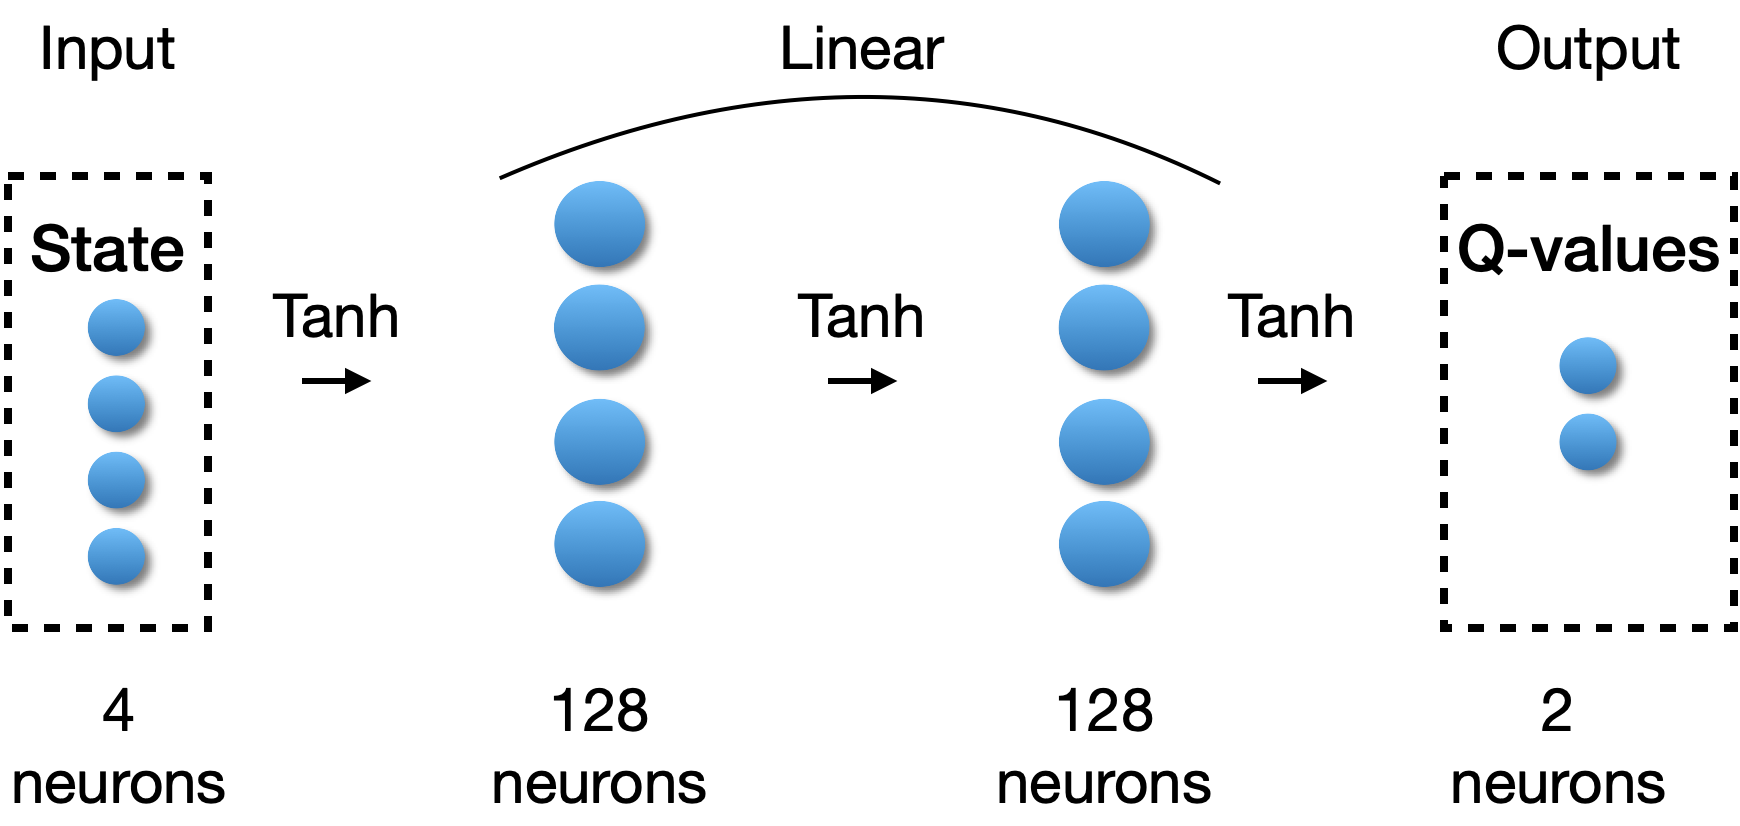
\includegraphics[width=0.6\textwidth]{Images/DQNet.png}
    \caption{Neural network for the evaluation of the $Q$-values given the state.}
    \label{fig:dqnet}
\end{figure}


In the reward function it is added a linear penalty proportional to the distance from the center of the screen, due to a problematic behavior of the agent that tried to "exit" 
from the screen.

We will try to speed up convergence as much as possible, in particular optimizing:
\begin{itemize}
    \item the exploration profile, of which we will change the starting temperature. As cited before, we will add gaussian increment of temperature at random position 
        in the profile with probability $p=0.3$, to understand its effect on the optimization. The exploration profile will be made of $1000$ points;
    \item The discount rate $\gamma$;
    \item The target update time $\tilde{n}$;
    \item The learning rate $\lambda$;
    \item The mini-batch size.
\end{itemize}

\subsection{Results}

We immediately understand that the performances of the algorithm are strongly dependent on the hyperparameters. We can see in Figure \ref{fig:hyper} the 
hyperparameter search, where the first\_solved axis is defined as the first time at which the agent performs at least $490$ points. If the agent is not able 
to solve the environment then we assign a first\_solved value of $1000$. We can see that the best performing agents have a high learning rate $\lambda$, a high 
discount rate $\gamma$ and a frequent update of the target network.
To better understand the evolution of the training and the effect of the exploration profile we plot the exploration profile and the training score, i.e. the score 
along all the points of the exploration. Obviously, they have different magnitudes, and so we will refer to the left axis for the exploration profile and to 
the right axis for the training score. The training score oscillates a lot along the evolution. We will so take an average each $20$ time step, taking as relative time step 
the central one. We see in Figure \ref{fig:best_cart} the best performing hyperparameters, in Figure \ref{fig:norm_cart} a good hyperparameter set and in Figure \ref{fig:bad_cart}
a set which is not able to solve the environment. The figures show clearly that, when the hyperparameter set is optimal, the score abruptly increases as soon as the 
temperature approaches zero, i.e. when the agent starts to choose the best action. This means that the learning is really fast. 
A bad choice can instead damage the learning so much that the agent is never able to solve the environment.

\section{Cartpole with pixels \label{sec:pixels}}
\subsection{Methods}
The aim of this section is again to solve the environment of the Cartpole from the gym library. However, we will not use the 
observation space described in the previous section. We will instead use the cartpole displayed in a screen.
This task is far from easy, since the agent now have to infer the previous observation space from images. We first
decrease the size of the observation space, which is a $600\times400$ RGB image, as follows:
\begin{itemize}
    \item We transform the image in grayscale, passing from $3$ channels to $1$;
    \item We crop the image such that we have a small amount of empty screen, while still leaving to the cart the possibility
        of moving and being observed. In particular, we crop $150$ pixels from the bottom, $80$ from the top, $200$ from the left
        and $200$ from the right.
\end{itemize}
We so end up with a $200\times170$ grayscale image, as shown in Figure \ref{fig:image}. Still, we do not have any means of understanding
information about the velocity from a single image. We so concatenate $4$ subsequent images as input of the network. 

Since we fed images to the agent, in this case we decided to use a convolutional neural network, which architecture is presented in Figure
\ref{fig:conv}.
\begin{figure}[h]
    \centering
    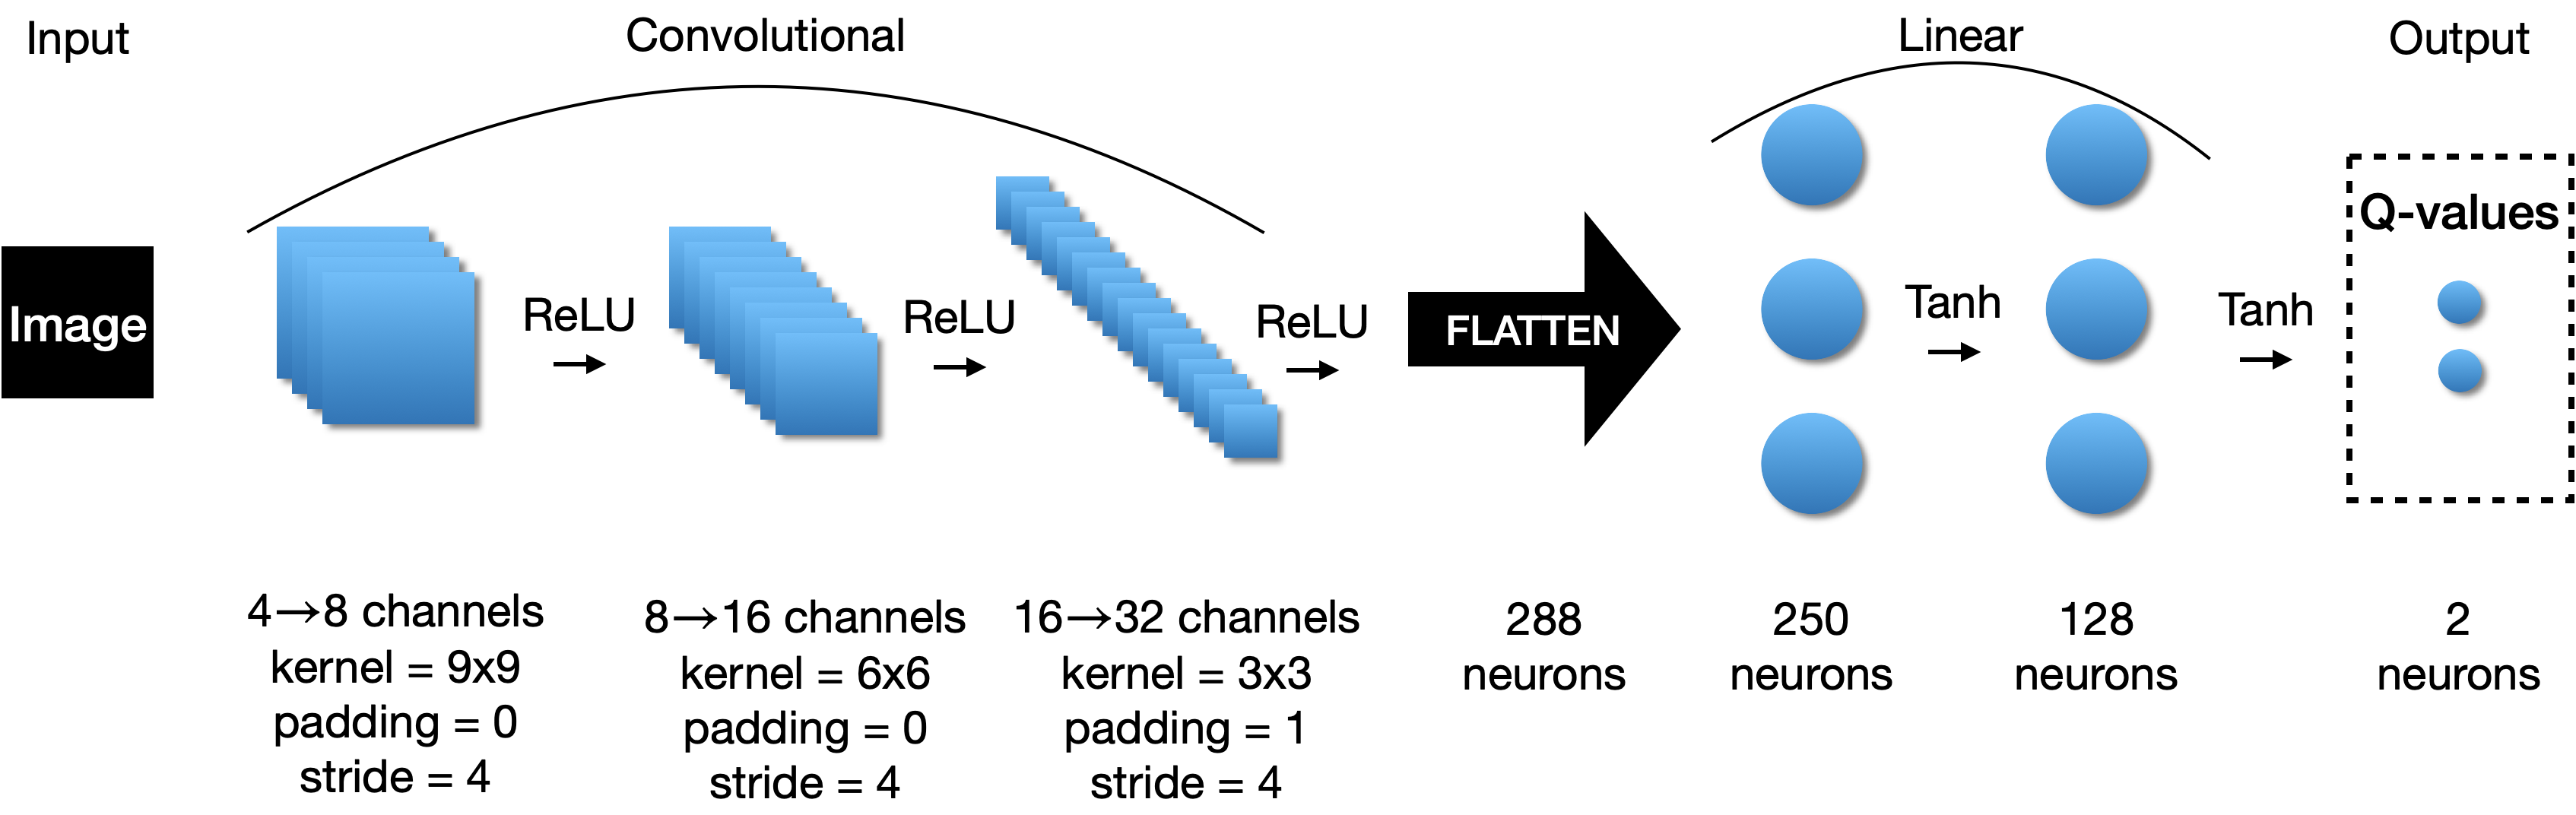
\includegraphics[width=0.7\textwidth]{Images/conv.png}
    \caption{Architecture of the convolutional neural network used as agent.}
    \label{fig:conv}
\end{figure}
It is important to notice that in the network we make plenty of use of the stride, which reduces the size of the image.

The firsts attempts were so difficult and low-performing that we thought of a trick to implement, divided into three main points:
\begin{itemize}
    \item Run the normal training, as in the previous section, but using the new observation space. Store the couples $[obs, st]$, where 
        $obs$ is given by the $4$ subsequent images defined above and $st$ is the state defined in Section \ref{sec:cart};
    \item Train a supervised convolutional neural network to predict $st$ given the $obs$, with the same structure shown in Figure \ref{fig:conv}, but where 
        the output layer has $4$ neurons instead of $2$;
    \item Perform transfer learning, by freezing the weights of the supervised network and attach to it a network with the same structure of Figure \ref{fig:dqnet}, and run
        the training again.
\end{itemize} 
This approach is particularly challenging due to the size of the $obs$, which quickly filled the RAM. It is however an interesting idea, and so we decided to present it 
anyway. 


\subsection{Results}
We used the best hyperparameter set found in the previous Section. As we can see in Figure \ref{fig:bef_trick} the network is able to learn a strategy to improve 
its score, thanks to all the tricks defined above. However, it is not able to solve the environment. We so decided to try to implement the procedure described 
above, adding a supervised part. The results of such a procedure are shown in Figure \ref{fig:aft_trick}. As we can observe, the results are worse than in the previous 
case, even if there is a learning. These results can be due to various problems of this task, first of all the scarcity of training samples for the supervised part,
on the order of $10\,000$, and not iid. Since the supervised part was not predicting the correct state the additional network was not able to produce meaningful
q-values.

We finally try to apply the same trick as above, but without freezing the weights of the previously trained network. The outcome is shown in Figure \ref{fig:nofreeze}. 
The learning is very unstable, and even if we manage to reach peaks of $200$ it is not clear if the performances really improve, or it is just a fluctuation.

\section{Lunar Landing \label{sec:LunLand}}
\subsection{Methods}
We choose to study the Lunar Lander environment from the gym library. It is slightly more difficult than the cartpole, since it has a larger 
observation space.
The observation space is the following:
$$
O = [x, y, v_x, v_y, \theta, \omega, l_l, l_r]
$$
where $x, y$ are the spatial coordinates, $v_x, v_y$ the velocities, $\theta$ the angle of the lander and $\omega$ its angular velocity. $l_l$
and $l_r$ are boolean variables and are True if the left (right) leg is in contact with the ground. The action space is instead:
$$
A = [null, l_e, c_e, r_e]
$$ 
where $null$ is “do nothing”, $l_e$ is “fire the left engine” and the last two action are respectively fire the central and right engine. The 
fuel is infinite.

The Landing pad starts always at coordinates $(0,0)$. The reward for moving from the top of the screen to landing pad with zero speed is about 
$100-140$ points. If the lander moves away from landing pad it loses reward back. An episode finishes 
if the lander crashes or comes to rest, receiving additional -100 or +100 points. Each leg which makes ground contact is $+10$ reward. 
Firing main engine is $-0.3$ points each frame. The environment is considered solved if the agent reaches $200$ points. 
It is possible to land outside the pad. We show an example of the rendered environment in Figure \ref{fig:Lunar}.

We will use all the tricks explained in Section \ref{sec:cart}.
Since the environment is slightly more difficult than the previous one, we will add another linear layer in the network, using the architecture 
presented in Figure \ref{fig:lun_arc}.
\begin{figure}
    \centering
    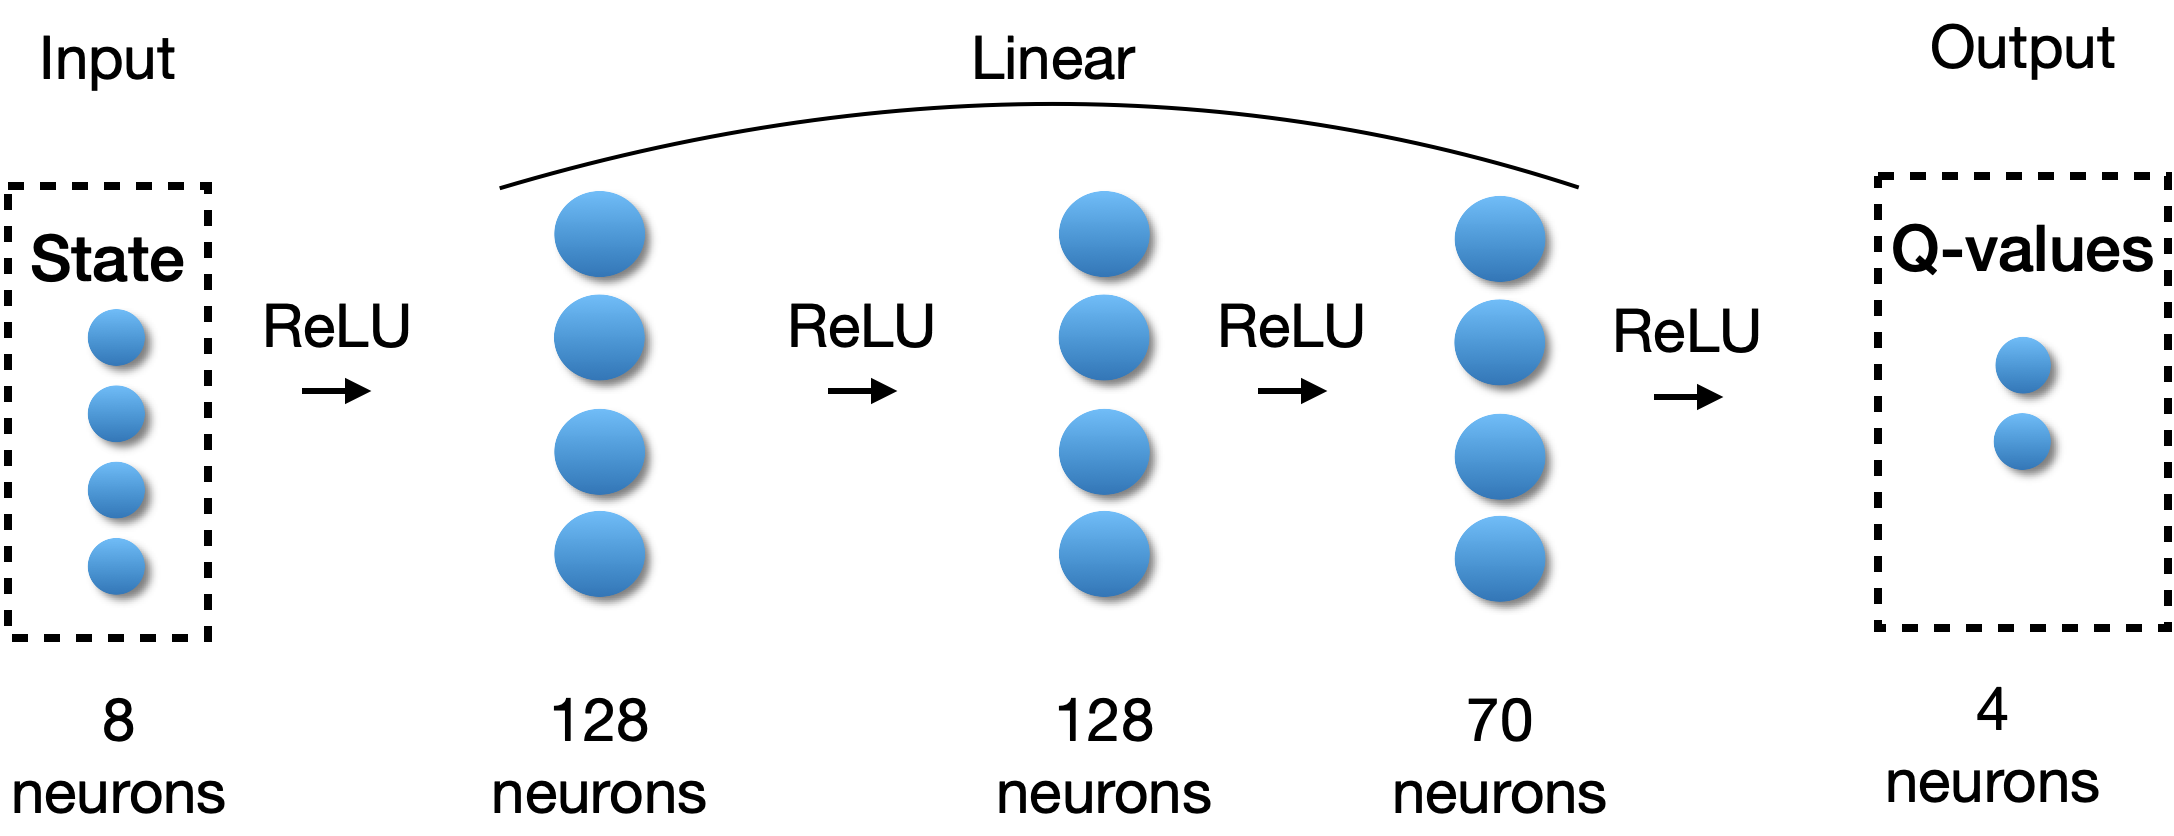
\includegraphics[width=0.7\textwidth]{Images/LunarLandNet.png}
    \caption{Architecture of the network used in the Lunar Lander environment.}
    \label{fig:lun_arc}
\end{figure}


\subsection{Results}
This environment was not trivial to solve. Indeed, to speed up convergence we tried to tweak the reward function. First, we gave some linear malus
if the lander moved away from the center of the screen, i.e.
$$
malus = -\eta |x|
$$
Even though the lander remained in the center of the screen it learned to fly indefinitely. Instead, adding a linear bonus for going downward, i.e.
$$
bonus = -\alpha v_y \theta(-v_y),
$$ 
where $\theta(t)$ is the Heaviside function and $alpha$ is a parameter set to $1.5$, helped in the convergence. In particular, we observe the average score and the exploration path in 
Figure \ref{fig:score_lunar}, and we can observe that it solves the environment at about $800$ steps. We can also observe that the score increases significantly at $600$ iterations after
a plateau, in correspondence to the end of the gaussian addition. This suggests that the increase in the temperature helped to discover a new strategy that was the correct one to solve the 
environment. We can so state that increasing the temperature at later stages of the learning may be useful to improve the final score.


\printbibliography

\newpage
\section{Appendix \label{sec:app}}
We present here images that can be interesting but are not fundamental for the report.
\begin{figure}[h]
    \centering
    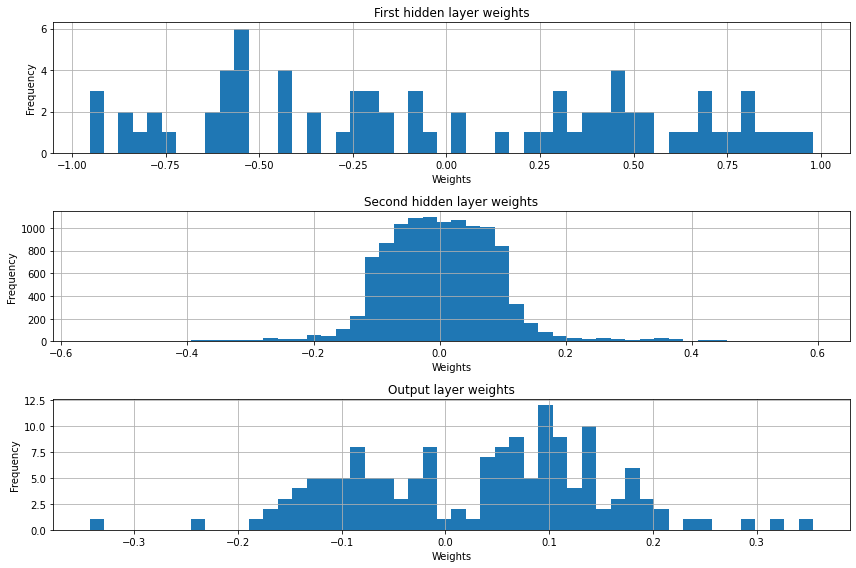
\includegraphics[width=0.8\textwidth]{Images/reg_weights.png}
    \caption{Weight histograms for the different layers of the network.}
    \label{fig:reg_weights}
\end{figure}

\begin{figure}[h]
    \centering
    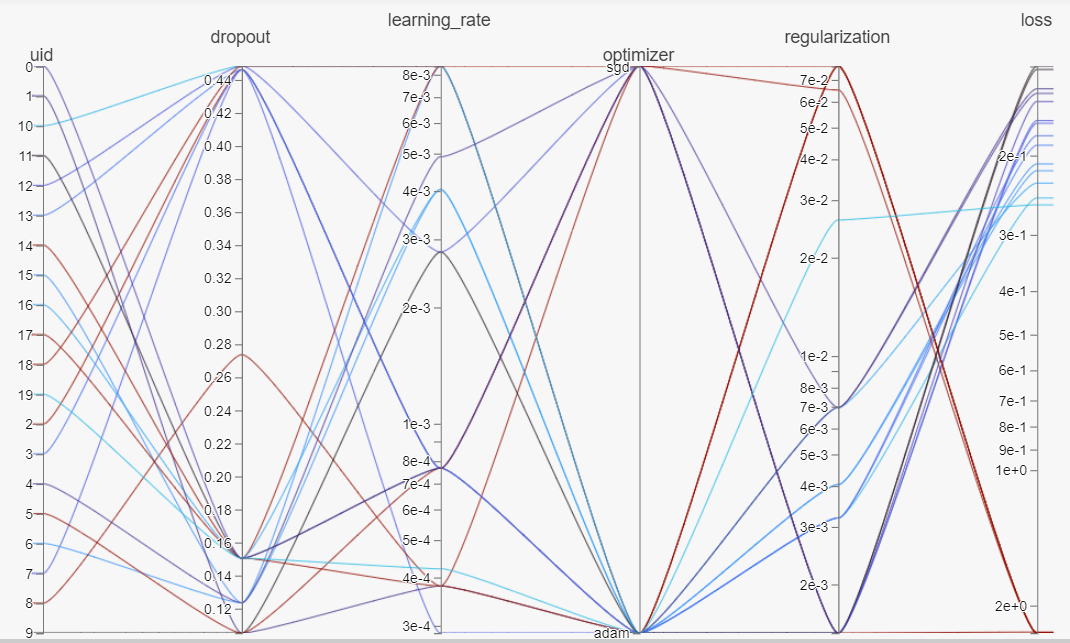
\includegraphics[width=0.8\textwidth]{Images/hyperparams.PNG}
    \caption{Hyperparameters search for the classification task. We plotted with a color which is proportional to the loss function,
    reported in log-scale. The darker the color, the better the result. We notice that a really high L2 regularization 
    usually translates in a low loss score.}
    \label{fig:cl_hp}
\end{figure}

%\end{multicols}



\end{document}
